\documentclass[tikz, border=10pt]{standalone}
\usetikzlibrary{shapes,fit}

\tikzset{
    pics/vhsplit/.style n args = {6}{
        code = {
        \draw [draw] (0,1) rectangle (1.25,0.5);
        \node[draw=none] at (0.625,0.75) {#1};
        \draw [draw] (1.25,1) rectangle (2,0.5);
        \node[draw=none] at (1.625,0.75) {#2};
        \draw [draw] (0,0.5) rectangle (0.5,0);
        \draw [draw] (0.5,0.5) rectangle (1,0);
        \draw [draw] (1,0.5) rectangle (1.5,0);
        \draw [draw] (1.5,0.5) rectangle (2,0);
        \node[draw=none] at (0.25,0.25) {\tiny{#3}};
        \node[draw=none] at (0.75,0.25) {\tiny{#4}};
        \node[draw=none] at (1.25,0.25) {\tiny{#5}};
        \node[draw=none] at (1.75,0.25) {\tiny{#6}};
        }
    }
}


\begin{document}
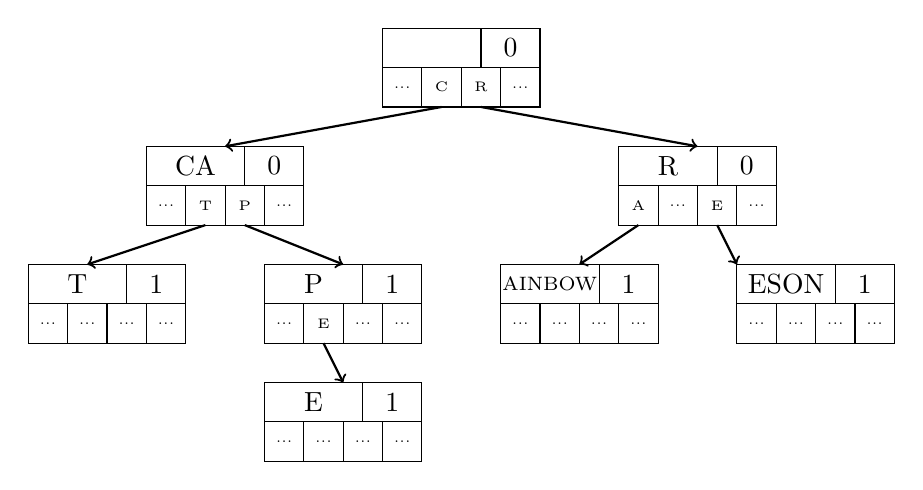
\begin{tikzpicture}%[every node/.append style={draw, rounded corners, inner sep=10pt}]
    \path pic {vhsplit={}{0}{...}{C}{R}{...}};
    \coordinate(CAs) at (0.75,0);
    \coordinate(Rs) at (1.25,0);

    \path pic at (-3,-1.5) {vhsplit={CA}{0}{...}{T}{P}{...}};
    \coordinate(CAn) at (-2,-0.5);
    \coordinate(Ts) at (-2.25,-1.5);
    \coordinate(Ps) at (-1.75,-1.5);

    \path pic at (-4.5,-3) {vhsplit={T}{1}{...}{...}{...}{...}};
    \coordinate(Tn) at (-3.75,-2);

    \path pic at (-1.5,-3) {vhsplit={P}{1}{...}{E}{...}{...}};
    \coordinate(Pn) at (-0.5,-2);
    \coordinate(Es) at (-0.75,-3);

    \path pic (E) at (-1.5,-4.5) {vhsplit={E}{1}{...}{...}{...}{...}};
    \coordinate(En) at (-0.5,-3.5);

    \draw [->,  thick] (CAs)--(CAn);
    \draw [->,  thick] (Ts)--(Tn);
    \draw [->,  thick] (Ps)--(Pn);
    \draw [->,  thick] (Es)--(En);

    \path pic at (3,-1.5) {vhsplit={R}{0}{A}{...}{E}{...}};
    \coordinate(Rn) at (4,-0.5);
    \coordinate(A1s) at (3.25,-1.5);
    \coordinate(E1s) at (4.25,-1.5);

    \path pic at (1.5,-3) {vhsplit={\scriptsize{AINBOW}}{1}{...}{...}{...}{...}};
    \coordinate(A1n) at (2.5,-2);

    \path pic at (4.5,-3) {vhsplit={ESON}{1}{...}{...}{...}{...}};
    \coordinate(E1n) at (4.5,-2);
    \coordinate(A2s) at (4.75,-3);

    \draw [->,  thick] (Rs)--(Rn);
    \draw [->,  thick] (A1s)--(A1n);
    \draw [->,  thick] (E1s)--(E1n);

\end{tikzpicture}
\end{document}
